\documentclass[border=4pt]{standalone}
\usepackage{tikz}
\usetikzlibrary{arrows,arrows.spaced,positioning}
\begin{document}
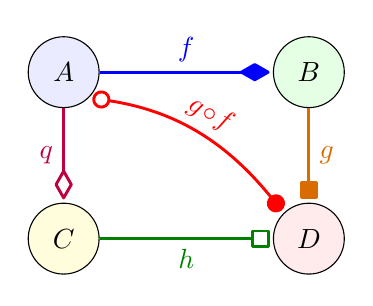
\begin{tikzpicture}[
  node distance=12mm and 22mm,
  object/.style={draw,circle,minimum size=9mm,inner sep=1pt},
  map/.style={line width=1.05pt}
]
  \node[object,fill=blue!8] (A) {$A$};
  \node[object,fill=green!10,right=of A] (B) {$B$};
  \node[object,fill=yellow!14,below=of A] (C) {$C$};
  \node[object,fill=red!8,right=of C] (D) {$D$};

  \draw[map,blue,-{spaced diamond}] (A) -- node[above] {$f$} (B);
  \draw[map,purple,-{spaced open diamond}] (A) -- node[left] {$q$} (C);
  \draw[map,orange!85!black,-{spaced square}] (B) -- node[right] {$g$} (D);
  \draw[map,green!50!black,-{spaced open square}] (C) -- node[below] {$h$} (D);
  \draw[map,red,{spaced o}-{spaced *}]
    (A.south east) to[bend left=22] node[above,sloped] {$g\!\circ\!f$} (D.north west);
\end{tikzpicture}
\end{document}
